% ============================================================
% LLM-BLM 実験 S3：リスクの読み取りで共分散を補正すると、BLM の TE の見積もりは正確になるか（事前登録した検定の結果）
% コンパイル：tectonic -X compile LLM-BLM_実験S3.tex   （XeTeX 系。このフォルダで実行する）
% 数値と表は 図/values.tex・図/tab_*.tex（作成スクリプト/values.py）、図は 図/*.pdf（作成スクリプト/figs.py）。
% どちらも experiments/S3_smallcap_risk_blm/results から作る。本文に数値を手で書かない。
% ============================================================
\documentclass[xelatex,ja=standard,jafont=haranoaji,a4paper,10pt,openany]{bxjsreport}
\setpagelayout*{left=22mm,right=22mm,top=24mm,bottom=26mm,footskip=11mm}

\usepackage{amsmath,amssymb,mathtools,bm}
\usepackage{booktabs,array,multirow,longtable}
\usepackage{graphicx}
\usepackage{adjustbox}
\usepackage{xcolor}
\usepackage{enumitem}
\usepackage{caption}
\usepackage{float}
\usepackage[most]{tcolorbox}
\usepackage[hidelinks,bookmarksnumbered]{hyperref}

\graphicspath{{図/}}
% values.py が results から作る。手で直さない。
\expandafter\def\csname v@commit\endcsname{a6107fb}
\expandafter\def\csname v@primaryD\endcsname{$+$0.0003}
\expandafter\def\csname v@primarylo\endcsname{$-$0.0004}
\expandafter\def\csname v@primaryhi\endcsname{$+$0.0012}
\expandafter\def\csname v@primaryp\endcsname{0.201}
\expandafter\def\csname v@primarybref\endcsname{1.220}
\expandafter\def\csname v@primarybnew\endcsname{1.219}
\expandafter\def\csname v@primarydays\endcsname{2,701}
\expandafter\def\csname v@BvsAD\endcsname{$+$0.0275}
\expandafter\def\csname v@BvsAlo\endcsname{$+$0.0103}
\expandafter\def\csname v@BvsAhi\endcsname{$+$0.0481}
\expandafter\def\csname v@BvsAp\endcsname{$<$0.001}
\expandafter\def\csname v@BvsAbref\endcsname{1.254}
\expandafter\def\csname v@BvsAbnew\endcsname{1.220}
\expandafter\def\csname v@BvsAdays\endcsname{2,701}
\expandafter\def\csname v@CvsAD\endcsname{$+$0.0278}
\expandafter\def\csname v@CvsAlo\endcsname{$+$0.0107}
\expandafter\def\csname v@CvsAhi\endcsname{$+$0.0485}
\expandafter\def\csname v@CvsAp\endcsname{$<$0.001}
\expandafter\def\csname v@CvsAbref\endcsname{1.254}
\expandafter\def\csname v@CvsAbnew\endcsname{1.219}
\expandafter\def\csname v@CvsAdays\endcsname{2,701}
\expandafter\def\csname v@gptCvsBD\endcsname{$+$0.0205}
\expandafter\def\csname v@gptCvsBlo\endcsname{$-$0.0057}
\expandafter\def\csname v@gptCvsBhi\endcsname{$+$0.0275}
\expandafter\def\csname v@gptCvsBp\endcsname{0.177}
\expandafter\def\csname v@gptCvsBbref\endcsname{2.175}
\expandafter\def\csname v@gptCvsBbnew\endcsname{2.131}
\expandafter\def\csname v@gptCvsBdays\endcsname{628}
\expandafter\def\csname v@primaryverdict\endcsname{支持されない}
\expandafter\def\csname v@usedB\endcsname{100\%}
\expandafter\def\csname v@usedC\endcsname{98\%}
\expandafter\def\csname v@usedCgpt\endcsname{75\%}
\expandafter\def\csname v@betaC\endcsname{$-$0.03}
\expandafter\def\csname v@betaCgpt\endcsname{$+$1.76}
\expandafter\def\csname v@B2015quarterchronoridgeA\endcsname{5.078}
\expandafter\def\csname v@X2015quarterchronoridgeA\endcsname{$+$2.8\%}
\expandafter\def\csname v@b2015quarterchronoridgeA\endcsname{1.25}
\expandafter\def\csname v@B2015quarterchronoridgeB\endcsname{5.171}
\expandafter\def\csname v@X2015quarterchronoridgeB\endcsname{$+$3.0\%}
\expandafter\def\csname v@b2015quarterchronoridgeB\endcsname{1.22}
\expandafter\def\csname v@B2015quarterchronoridgeC\endcsname{5.172}
\expandafter\def\csname v@X2015quarterchronoridgeC\endcsname{$+$3.0\%}
\expandafter\def\csname v@b2015quarterchronoridgeC\endcsname{1.22}
\expandafter\def\csname v@B2015quarterband\endcsname{3.906}
\expandafter\def\csname v@B2015halfchronoridgeA\endcsname{4.807}
\expandafter\def\csname v@X2015halfchronoridgeA\endcsname{$+$2.4\%}
\expandafter\def\csname v@b2015halfchronoridgeA\endcsname{1.28}
\expandafter\def\csname v@B2015halfchronoridgeB\endcsname{4.788}
\expandafter\def\csname v@X2015halfchronoridgeB\endcsname{$+$2.4\%}
\expandafter\def\csname v@b2015halfchronoridgeB\endcsname{1.26}
\expandafter\def\csname v@B2015halfchronoridgeC\endcsname{4.795}
\expandafter\def\csname v@X2015halfchronoridgeC\endcsname{$+$2.4\%}
\expandafter\def\csname v@b2015halfchronoridgeC\endcsname{1.26}
\expandafter\def\csname v@B2015halfband\endcsname{3.838}
\expandafter\def\csname v@B2015yearchronoridgeA\endcsname{4.732}
\expandafter\def\csname v@X2015yearchronoridgeA\endcsname{$+$1.6\%}
\expandafter\def\csname v@b2015yearchronoridgeA\endcsname{1.34}
\expandafter\def\csname v@B2015yearchronoridgeB\endcsname{4.782}
\expandafter\def\csname v@X2015yearchronoridgeB\endcsname{$+$1.7\%}
\expandafter\def\csname v@b2015yearchronoridgeB\endcsname{1.31}
\expandafter\def\csname v@B2015yearchronoridgeC\endcsname{4.785}
\expandafter\def\csname v@X2015yearchronoridgeC\endcsname{$+$1.7\%}
\expandafter\def\csname v@b2015yearchronoridgeC\endcsname{1.31}
\expandafter\def\csname v@B2015yearband\endcsname{4.065}
\expandafter\def\csname v@B2023quarterchronoridgeA\endcsname{1.873}
\expandafter\def\csname v@X2023quarterchronoridgeA\endcsname{$+$10.3\%}
\expandafter\def\csname v@b2023quarterchronoridgeA\endcsname{1.40}
\expandafter\def\csname v@B2023quarterchronoridgeB\endcsname{1.844}
\expandafter\def\csname v@X2023quarterchronoridgeB\endcsname{$+$9.6\%}
\expandafter\def\csname v@b2023quarterchronoridgeB\endcsname{1.30}
\expandafter\def\csname v@B2023quarterchronoridgeC\endcsname{1.844}
\expandafter\def\csname v@X2023quarterchronoridgeC\endcsname{$+$9.6\%}
\expandafter\def\csname v@b2023quarterchronoridgeC\endcsname{1.30}
\expandafter\def\csname v@B2023quartergptridgeA\endcsname{1.527}
\expandafter\def\csname v@X2023quartergptridgeA\endcsname{$+$1.3\%}
\expandafter\def\csname v@b2023quartergptridgeA\endcsname{2.49}
\expandafter\def\csname v@B2023quartergptridgeB\endcsname{1.538}
\expandafter\def\csname v@X2023quartergptridgeB\endcsname{$+$1.6\%}
\expandafter\def\csname v@b2023quartergptridgeB\endcsname{2.17}
\expandafter\def\csname v@B2023quartergptridgeCgpt\endcsname{1.539}
\expandafter\def\csname v@X2023quartergptridgeCgpt\endcsname{$+$1.7\%}
\expandafter\def\csname v@b2023quartergptridgeCgpt\endcsname{2.13}
\expandafter\def\csname v@B2023quarterband\endcsname{1.479}
\expandafter\def\csname v@B2023halfchronoridgeA\endcsname{1.766}
\expandafter\def\csname v@X2023halfchronoridgeA\endcsname{$+$6.9\%}
\expandafter\def\csname v@b2023halfchronoridgeA\endcsname{1.40}
\expandafter\def\csname v@B2023halfchronoridgeB\endcsname{1.766}
\expandafter\def\csname v@X2023halfchronoridgeB\endcsname{$+$6.9\%}
\expandafter\def\csname v@b2023halfchronoridgeB\endcsname{1.32}
\expandafter\def\csname v@B2023halfchronoridgeC\endcsname{1.766}
\expandafter\def\csname v@X2023halfchronoridgeC\endcsname{$+$6.9\%}
\expandafter\def\csname v@b2023halfchronoridgeC\endcsname{1.32}
\expandafter\def\csname v@B2023halfgptridgeA\endcsname{1.455}
\expandafter\def\csname v@X2023halfgptridgeA\endcsname{$-$1.5\%}
\expandafter\def\csname v@b2023halfgptridgeA\endcsname{2.61}
\expandafter\def\csname v@B2023halfgptridgeB\endcsname{1.451}
\expandafter\def\csname v@X2023halfgptridgeB\endcsname{$-$1.6\%}
\expandafter\def\csname v@b2023halfgptridgeB\endcsname{2.28}
\expandafter\def\csname v@B2023halfgptridgeCgpt\endcsname{1.453}
\expandafter\def\csname v@X2023halfgptridgeCgpt\endcsname{$-$1.6\%}
\expandafter\def\csname v@b2023halfgptridgeCgpt\endcsname{2.23}
\expandafter\def\csname v@B2023halfband\endcsname{1.508}
\expandafter\def\csname v@B2023yearchronoridgeA\endcsname{1.683}
\expandafter\def\csname v@X2023yearchronoridgeA\endcsname{$+$3.6\%}
\expandafter\def\csname v@b2023yearchronoridgeA\endcsname{1.51}
\expandafter\def\csname v@B2023yearchronoridgeB\endcsname{1.682}
\expandafter\def\csname v@X2023yearchronoridgeB\endcsname{$+$3.6\%}
\expandafter\def\csname v@b2023yearchronoridgeB\endcsname{1.46}
\expandafter\def\csname v@B2023yearchronoridgeC\endcsname{1.682}
\expandafter\def\csname v@X2023yearchronoridgeC\endcsname{$+$3.6\%}
\expandafter\def\csname v@b2023yearchronoridgeC\endcsname{1.45}
\expandafter\def\csname v@B2023yeargptridgeA\endcsname{1.470}
\expandafter\def\csname v@X2023yeargptridgeA\endcsname{$-$2.2\%}
\expandafter\def\csname v@b2023yeargptridgeA\endcsname{1.54}
\expandafter\def\csname v@B2023yeargptridgeB\endcsname{1.461}
\expandafter\def\csname v@X2023yeargptridgeB\endcsname{$-$2.5\%}
\expandafter\def\csname v@b2023yeargptridgeB\endcsname{1.42}
\expandafter\def\csname v@B2023yeargptridgeCgpt\endcsname{1.464}
\expandafter\def\csname v@X2023yeargptridgeCgpt\endcsname{$-$2.4\%}
\expandafter\def\csname v@b2023yeargptridgeCgpt\endcsname{1.39}
\expandafter\def\csname v@B2023yearband\endcsname{1.550}

\newcommand{\V}[1]{\ifcsname v@#1\endcsname\csname v@#1\endcsname\else\textbf{??#1??}\fi}
\newcommand{\tabin}[1]{\adjustbox{max width=\linewidth}{\input{図/tab_#1.tex}}}

\definecolor{c1}{HTML}{2A78D6}
\definecolor{c2}{HTML}{EB6834}
\definecolor{soft1}{HTML}{E4EEF9}
\definecolor{soft2}{HTML}{FBEEDF}

\newcommand{\code}[1]{\texttt{#1}}
\newcommand{\SP}{S\&P500}
\newcommand{\figref}[1]{図~\ref{#1}}
\newcommand{\tabref}[1]{表~\ref{#1}}
\newcommand{\chapref}[1]{第~\ref{#1}~章}

\setlist[itemize]{leftmargin=1.6em,itemsep=0.2em,topsep=0.4em}
\setlist[enumerate]{leftmargin=1.8em,itemsep=0.2em,topsep=0.4em}
\captionsetup{font=small,labelfont=bf,skip=6pt}
\renewcommand{\arraystretch}{1.2}

\makeatletter
\def\@makechapterhead#1{\vspace*{0.3\Cvs}{\parindent\z@\raggedright\normalfont
  \ifnum\c@secnumdepth>\m@ne\if@mainmatter{\Large\headfont\@chapapp\thechapter\@chappos}\par\nobreak\vskip0.4\Cvs\fi\fi
  \interlinepenalty\@M\LARGE\headfont #1\par\nobreak\vskip 1.5\Cvs}}
\def\@makeschapterhead#1{\vspace*{0.3\Cvs}{\parindent\z@\raggedright\normalfont
  \interlinepenalty\@M\LARGE\headfont #1\par\nobreak\vskip 1.5\Cvs}}
\makeatother

\newtcolorbox{keybox}[1][要点]{enhanced,breakable,colback=soft1,colframe=c1,boxrule=0.5pt,arc=2pt,
  left=8pt,right=8pt,top=6pt,bottom=6pt,title={#1},fonttitle=\sffamily\bfseries\small,coltitle=white}

\title{LLM-BLM 実験 S3\\[6pt]
  \large リスクの読み取りで共分散を補正すると、\\BLM の TE の見積もりは正確になるか}
\author{実験の報告書（事前登録した検定の結果）}
\date{2026 年 10 月 25 日}

\begin{document}
\maketitle

\chapter*{概要}
\addcontentsline{toc}{chapter}{概要}

実験 S2 で、決算発表文のリスクの読み取りは、発表後の変動率を（小さいが）予測した。この実験 S3 では、その点数で銘柄の分散を相対的に補正した共分散を使い、S1 のリターンの見通しと組み合わせた BLM を作った。リスクの見積もりが正確になるかを事前登録して検定し、2015 年末と 2023 年末を 1 とした四半期・半年・1 年ごとの推移を報告した。gpt-4o-mini の版も並べた。

\begin{keybox}[要点]
\begin{itemize}
\item \textbf{主な検定は\V{primaryverdict}}。テキストのリスクの点数を足しても（C）、株価だけで補正した場合（B）より、TE の見積もりの偏りは小さくならなかった（偏り $b$ は \V{primarybref} から \V{primarybnew}、片側 $p$ = \V{primaryp}）。補正の回帰の中で、ChronoGPT のリスクの点数にはほとんど重みがつかなかった。
\item \textbf{株価による補正ははっきり効いた}（副次）。発表の後の銘柄の分散を、直近の変動率と 2 日の反応の大きさで補正すると、偏りは \V{BvsAbref} から \V{BvsAbnew} に小さくなり（95\% 区間が 0 を含まない）、すべての組み合わせで改善した。
\item \textbf{それでも事前の TE は小さすぎる}。どの組み合わせでも $b > 1$ で、gpt-4o-mini の見通しの BLM では、四半期・半年ごとで 2 を超えた。
\item \textbf{推移は 3 つの版でほぼ同じ}。ChronoGPT の見通しの BLM は、どの版・どの頻度でも比べる相手を上回った（2015 年末から四半期ごとで、最終の値は A が \V{B2015quarterchronoridgeA}、C が \V{B2015quarterchronoridgeC}、比べる相手が \V{B2015quarterband}）。
\item \textbf{注意}：S1・S2 と同じ 1,000 社で、その結果を見た後に設計した。資産の水準は生存者バイアスで高く出ている。
\end{itemize}
\end{keybox}


\setcounter{tocdepth}{1}
{\small\tableofcontents}

% ============================================================
\chapter{目的}\label{ch:purpose}

\begin{itemize}
\item 実験 S1：小型株で、ChronoGPT＋リッジのリターンの点数は、発表後 2〜60 日のドリフトを予測した。その点数を見通しにした BLM（追記 1）は、比べる相手を上回ったが、実現の TE は事前の上限（年 3\%）を超えた。
\item 実験 S2：ChronoGPT＋リッジのリスクの点数は、発表後の変動率を、過去の変動率を超えて予測した。ただし大きさは小さく、情報は「同じ時期の銘柄どうしの相対的なリスク」についてのものだった。
\end{itemize}

そこで、リスクの読み取りで銘柄の分散を相対的に補正し、S1 のリターンの見通しと組み合わせた BLM を作った。

\begin{keybox}[問い]
リスクの点数で共分散を補正すると、BLM のポートフォリオの事前の TE は、実現の TE をより正確に見積もるようになるか。あわせて、その BLM の資産の推移はどうなるか。
\end{keybox}

% ============================================================
\chapter{事前登録}\label{ch:prereg}

仮説・方法・判定の基準は \code{experiments/S3\_smallcap\_risk\_blm/preregistration.md} に書き、コード（\code{run.py}）と同じコミットで固定してから、1 回だけ実行した。実行に使ったコミットは \code{\V{commit}}。

\begin{itemize}
\item \textbf{同じ標本}：S1・S2 と同じ 1,000 社で、S1・S2 の結果を見た後に設計した。S3 の結果は、S2 の結果（リスクの点数が変動率を予測すること）を前提にしている。
\item \textbf{計算していなかったもの}：補正した共分散による BLM の比率・推移・TE は、どれも計算していなかった。
\end{itemize}

% ============================================================
\chapter{方法}\label{ch:method}

\section{ポートフォリオ}

範囲、リバランスの日（四半期・半年・1 年ごと）、始点（2015 年 12 月末と 2023 年 12 月末を 1 とする）、見通しの作り方、BLM（$\delta = 2.5$、$\tau = 0.025$、He--Litterman の $\Omega$、IC $= 0.05$）、事前の TE の上限（年 3\%）、費用（片道 0.3\%）、比べる相手（範囲を浮動株時価総額で加重）は、S1 の追記 1 と同じにした。違うのは共分散だけである。

\section{共分散の 3 つの版}

各リバランスの日に、直近 252 日の Ledoit--Wolf の共分散 $\Sigma$ を作り、銘柄ごとの倍率 $s_i$ で $\Sigma' = S\Sigma S$（$S = \mathrm{diag}(s)$。分散を変え、相関の形は保つ）とした。$\Sigma'$ を、均衡のリターン（$\delta\Sigma' w$）、$\Omega$、見通しの $\sigma$、最適化と TE のすべてに使った。倍率は、その日以前の 60 取引日以内に発表があった銘柄にだけかけた。

\begin{table}[H]
\centering\small
\caption{共分散の 3 つの版}
\label{tab:versions}
\begin{tabular}{@{}lp{0.72\linewidth}@{}}
\toprule
版 & 倍率 \\
\midrule
A 基準 & $s = 1$（追記 1 と同じ） \\
B 株価で補正 & 過去の発表（その日より前に 60 日の窓が閉じたもの）で、発表後 2〜60 日の対数の変動率を、発表の前の変動率・規模・2 日の反応の大きさ・驚きの大きさに、年・四半期の中で平均を引いて回帰する。その日の発表の後の銘柄の、予測した相対的な変動率と、Ledoit--Wolf の相対的な変動率の比を倍率にする（$[0.5, 2]$ に丸める） \\
C 株価＋テキスト & B の説明変数に、リスクの点数（ChronoGPT：S2 の \code{chrono\_risk}、gpt-4o-mini の版は \code{gpt\_risk}）を足す。点数のない銘柄は B の倍率 \\
\bottomrule
\end{tabular}
\end{table}

\section{主な検定}

2015 年末から四半期ごとにリバランスする、ChronoGPT＋リッジの見通しの BLM で、日次の超過リターン（ポートフォリオ − 比べる相手）を、直近のリバランスの日の事前の日次の TE（その版の $\Sigma'$ で計算）で割った $z_t$ を作る。偏りの統計量 $b = \sqrt{\overline{z_t^2}}$ は、$b = 1$ なら事前の TE が実現の TE を正しく見積もっていることを表す。

\begin{itemize}
\item \textbf{P}：$D = |\log b_B| - |\log b_C| > 0$（C のほうが 1 に近い）か。
\item \textbf{判定}：ブロックの長さ 63 日の円形のブロック・ブートストラップ（B と C の同じ日を一緒に引く、2,000 回）で、$D^* \leq 0$ の割合を片側 $p$ とし、$p < 0.05$ なら「支持」。
\item \textbf{副次}：B と A、C と A（同じ形）、gpt-4o-mini の版（2023 年末から四半期ごと、C と B）。資産の推移は報告だけ。
\end{itemize}

% ============================================================
% 結果の章（数値は 図/values.tex と 図/tab_*.tex から。手で書かない）

% ============================================================
\chapter{主な検定}\label{ch:primary}

\begin{table}[H]
\centering\small
\caption{TE の見積もりの偏り（2015 年末から、四半期ごと、ChronoGPT＋リッジの見通し、\V{primarydays} 日）}
\label{tab:tests}
\begin{tabular}{@{}lrrrrr@{}}
\toprule
比べたもの & $b$（前） & $b$（後） & $D$ & 95\% 区間 & 片側 $p$ \\
\midrule
\textbf{主：C（株価＋テキスト）と B（株価）} & \V{primarybref} & \V{primarybnew} & \V{primaryD} & [\V{primarylo}, \V{primaryhi}] & \V{primaryp} \\
副：B（株価）と A（基準） & \V{BvsAbref} & \V{BvsAbnew} & \V{BvsAD} & [\V{BvsAlo}, \V{BvsAhi}] & \V{BvsAp} \\
副：C（株価＋テキスト）と A（基準） & \V{CvsAbref} & \V{CvsAbnew} & \V{CvsAD} & [\V{CvsAlo}, \V{CvsAhi}] & \V{CvsAp} \\
副：gpt-4o-mini、C と B（2023 年末から、\V{gptCvsBdays} 日） & \V{gptCvsBbref} & \V{gptCvsBbnew} & \V{gptCvsBD} & [\V{gptCvsBlo}, \V{gptCvsBhi}] & \V{gptCvsBp} \\
\bottomrule
\end{tabular}
\end{table}

$b$ は偏りの統計量（日次の超過リターン ÷ 事前の TE の 2 乗平均の平方根。1 なら事前の TE が正しい）。$D = |\log b_{\text{前}}| - |\log b_{\text{後}}|$ が正なら、後の版のほうが 1 に近い。

\begin{keybox}[結果]
主な検定は\textbf{\V{primaryverdict}}。テキストのリスクの点数を足しても、TE の見積もりの偏りはほとんど変わらなかった（$b$ は \V{primarybref} から \V{primarybnew}、片側 $p$ = \V{primaryp}）。一方、副次の検定では、\textbf{株価のデータによる補正（B）が、偏りをはっきり小さくした}（$b$ は \V{BvsAbref} から \V{BvsAbnew}、95\% 区間が 0 を含まない）。
\end{keybox}

\begin{itemize}
\item \textbf{テキストの点数の重み}：C の補正の回帰で学習されたリスクの点数の係数は、リバランスの日の平均で、1 標準偏差あたり変動率の \V{betaC}\%（ChronoGPT）だった。株価のデータの説明変数を入れた補正の回帰の中では、ChronoGPT のリスクの点数にはほとんど重みがつかず、C は B とほぼ同じになった。gpt-4o-mini の点数の係数は \V{betaCgpt}\% だった。
\item \textbf{補正をかけた日の割合}：B は \V{usedB}、C は \V{usedC}、gpt-4o-mini の C は \V{usedCgpt}（学習の発表が足りない日は B の倍率を使った）。
\end{itemize}

% ============================================================
\chapter{すべての組み合わせ}\label{ch:runs}

\section{偏りの統計量}

\begin{figure}[H]
\centering
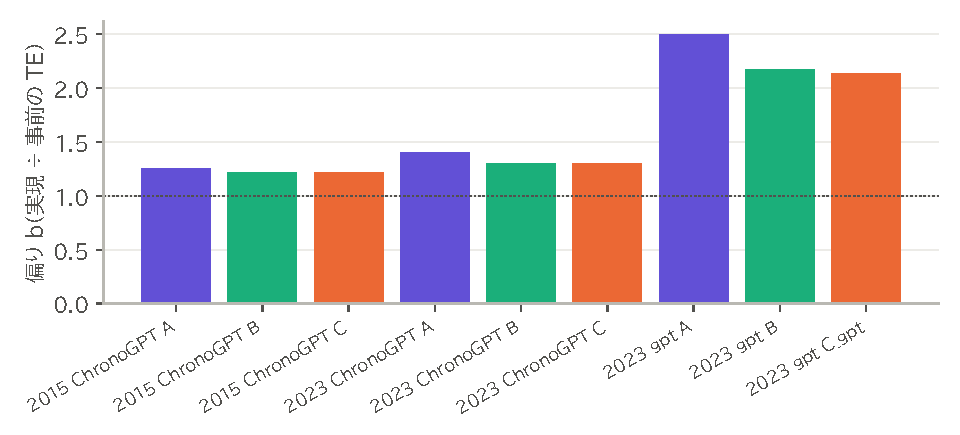
\includegraphics[width=0.8\linewidth]{bias.pdf}
\caption{四半期ごとのリバランスの、版ごとの偏り $b$。点線は 1（事前の TE が正しい）。}
\label{fig:bias}
\end{figure}

\begin{itemize}
\item どの組み合わせでも $b > 1$ で、事前の TE は実現の TE を\textbf{小さく見積もっていた}。S1 の追記 1 で見た「実現の TE が上限を超える」問題が、ここでも確かめられた。
\item 株価による補正（B）は、2015 年末から・2023 年末から、ChronoGPT・gpt-4o-mini の見通し、四半期・半年・1 年のどの組み合わせでも、偏りを A より小さくした（\tabref{tab:runs2015}・\tabref{tab:runs2023}）。テキストを足した C は、B とほとんど同じだった。
\item gpt-4o-mini の見通しの BLM は、偏りが特に大きい（四半期・半年ごとでは $b$ が 2 を超える）。事前の TE は年 2〜3\% だが、四半期・半年ごとでは実現の TE がその 2 倍前後だった。
\end{itemize}

\section{2015 年末から}

\begin{table}[H]
\centering\small
\caption{2015 年 12 月末を 1 とした推移（2026 年 9 月末まで）。年率と相手との差は年率、TE は年率、回転率はリバランス 1 回あたり}
\label{tab:runs2015}
\tabin{runs_2015}
\end{table}

\begin{figure}[H]
\centering
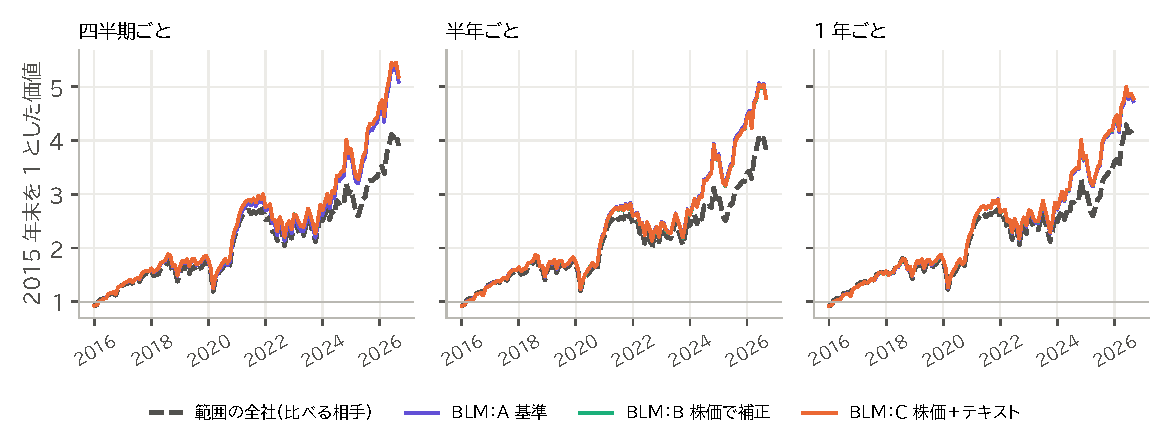
\includegraphics[width=\linewidth]{paths_2015_chrono_ridge.pdf}
\caption{2015 年末を 1 とした推移（ChronoGPT＋リッジの見通し）。3 つの版の線はほぼ重なる。}
\label{fig:paths2015}
\end{figure}

\section{2023 年末から}

\begin{table}[H]
\centering\small
\caption{2023 年 12 月末を 1 とした推移（2026 年 9 月末まで、約 2 年 9 か月）}
\label{tab:runs2023}
\tabin{runs_2023}
\end{table}

\begin{figure}[H]
\centering
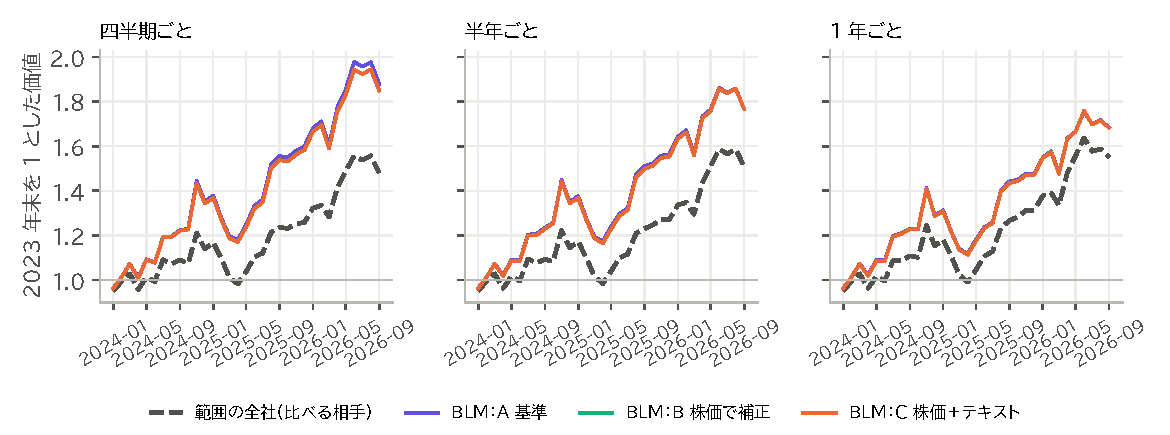
\includegraphics[width=\linewidth]{paths_2023_chrono_ridge.pdf}
\caption{2023 年末を 1 とした推移（ChronoGPT＋リッジの見通し）。}
\label{fig:paths2023c}
\end{figure}

\begin{figure}[H]
\centering
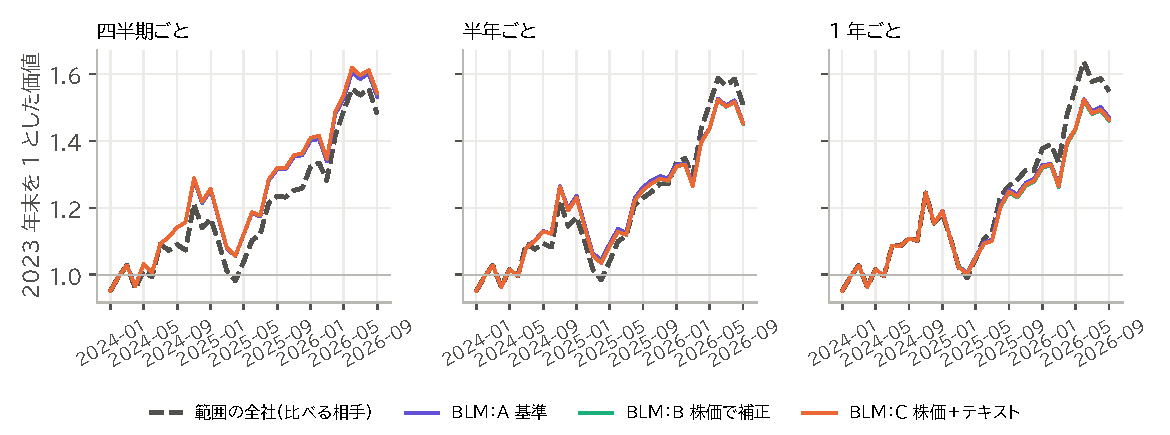
\includegraphics[width=\linewidth]{paths_2023_gpt_ridge.pdf}
\caption{2023 年末を 1 とした推移（gpt-4o-mini（重みを学習）の見通し）。}
\label{fig:paths2023g}
\end{figure}

\begin{itemize}
\item 推移は、3 つの版でほぼ重なった。共分散の補正は、リターンにはほとんど影響しない。2015 年末から四半期ごとでは、最終の値は A が \V{B2015quarterchronoridgeA}、B が \V{B2015quarterchronoridgeB}、C が \V{B2015quarterchronoridgeC}（比べる相手は \V{B2015quarterband}）。
\item ChronoGPT＋リッジの見通しの BLM は、どの版でも、2015 年末から・2023 年末からの両方で、比べる相手を上回った（S1 の追記 1 と同じ）。gpt-4o-mini（重みを学習）の見通しは、四半期ごとではわずかに上回り、半年・1 年ごとでは下回った。
\item 資産の水準は、生存者バイアスで高く出ている。意味があるのは差だけである。
\end{itemize}

% ============================================================
\chapter{解釈}\label{ch:interpret}

\section{何が分かったか}

\begin{enumerate}
\item \textbf{テキストのリスクの点数で共分散を補正しても、BLM のリスクの見積もりは良くならなかった}。S2 で見たテキストの効果は小さく、株価のデータ（発表の前の変動率、2 日の反応の大きさ）と一緒に補正の回帰に入れると、ChronoGPT のリスクの点数にはほとんど重みがつかなかった。S2 の結論（「予測の力はあるが、大きさは小さく、水準の予測には役立たない」）と一致する。
\item \textbf{株価のデータによる補正は、リスクの見積もりをはっきり良くした}。発表の後の銘柄の分散を、直近の変動率と反応の大きさで相対的に補正するだけで、すべての組み合わせで偏りが小さくなった。決算の後のリスクの変化は、直近 252 日の共分散では捉えきれない。
\item \textbf{それでも事前の TE は小さすぎる}。補正しても $b$ は ChronoGPT の見通しで 1.2〜1.5、gpt-4o-mini の見通しで 1.4〜2.3 で、実現の TE は事前の上限を 2 割以上超えた。最適化は、推定の誤差で小さく見積もられたリスクの方向に比率を寄せやすい（平均分散の「誤差の最大化」、ヘッジファンドの報告書の第 7 章）。共分散の推定（500 銘柄前後を 252 日で）の誤差と、小型株の固有の変動の急な変化が、その原因の候補である。
\item \textbf{推移はほとんど変わらなかった}。共分散の補正は、TE の配分を少し動かすだけで、リターンの大きさは見通しで決まる。
\end{enumerate}

\section{次に試すこと}

\begin{itemize}
\item \textbf{TE の校正}：過去の偏り $b$ で事前の TE の上限を割り引く（実験 X03 の考え方。上限 3\% なら、$b = 1.2$ のとき事前の上限を 2.5\% にする）。
\item \textbf{共分散の推定}：ファクター型のリスクモデル（業種・規模・モメンタムなど）や、より強い縮小。株価による補正（B）は残す。
\item \textbf{gpt-4o-mini の見通しの偏りの理由}：見通しがどの銘柄・どのリスクに偏っているかを調べる（探索）。
\item \textbf{テキストのリスクの点数}は、共分散の補正ではなく、S2 で効いた「2 日の反応の大きさ」の予測（決算の前後の量の調整）に使う方が筋がよいかもしれない。
\end{itemize}


% ============================================================
\chapter{限界}\label{ch:limits}

\begin{itemize}
\item \textbf{同じ 1,000 社}：S1・S2 と同じ標本で、今も上場している会社だけである。別の会社での確認は、まだしていない。
\item \textbf{推移は 1 回の実現}：TE 3\% の違いを、推移の差で見分ける検出力は低い。
\item \textbf{倍率の期間}：倍率は発表後 60 日の変動率の予測から作るが、保有期間（四半期・半年・1 年）とは一致しない。
\item \textbf{gpt-4o-mini の期間は短い}：2023 年末からの約 2 年 9 か月で、gpt-4o-mini のリスクの点数で補正できるのは、学習の発表が十分にたまった後だけである。
\end{itemize}

% ============================================================
\chapter*{再現の手順}
\addcontentsline{toc}{chapter}{再現の手順}

リポジトリの直下で（\code{.venv} の Python）、S1 と S2 の \code{run.py} の後に：

\begin{enumerate}
\item \code{python experiments/S3\_smallcap\_risk\_blm/run.py}（結果は \code{results/}。2 回目は summary.json があると止まる）。
\item \code{資料集/02\_実験/実験S3\_リスクで補正したBLM/作成スクリプト/} の \code{values.py} と \code{figs.py}。
\item このフォルダで \code{tectonic -X compile LLM-BLM\_実験S3.tex}。
\end{enumerate}

\end{document}
